\documentclass{beamer}

\usetheme{default}
\usepackage{helvet}
\usepackage[utf8]{inputenc}
\usepackage{hyperref,xspace,multicol}
\usepackage[absolute,overlay]{textpos}
\usepackage{tikz}
\usetikzlibrary{arrows,shapes,trees,shadows,positioning}
\usepackage{tree}
\usepackage{fancyvrb}           % for \Verb

% Remember the position of every picture.
\tikzstyle{every picture}+=[remember picture]

\tikzset{onslide/.code args={<#1>#2}{%
  \only<#1>{\pgfkeysalso{#2}} % \pgfkeysalso doesn't change the path
}}

% Colors.
\definecolor{guixred1}{RGB}{226,0,38}  % red P
\definecolor{guixorange1}{RGB}{243,154,38}  % guixorange P
\definecolor{guixyellow}{RGB}{254,205,27}  % guixyellow P
\definecolor{guixred2}{RGB}{230,68,57}  % red S
\definecolor{guixorange2}{RGB}{236,117,40}  % guixorange S
\definecolor{guixtaupe}{RGB}{134,113,127} % guixtaupe S
\definecolor{guixgrey}{RGB}{91,94,111} % guixgrey S
\definecolor{guixblue1}{RGB}{38,109,131} % guixblue S
\definecolor{guixblue2}{RGB}{28,70,114} % guixblue S
\definecolor{guixgreen1}{RGB}{133,146,66} % guixgreen S
\definecolor{guixgreen2}{RGB}{157,193,7} % guixgreen S

% White-on-black color theme.
\setbeamercolor{structure}{fg=guixorange1,bg=black}
\setbeamercolor{title}{fg=white,bg=black}
\setbeamercolor{date}{fg=guixorange1,bg=black}
\setbeamercolor{frametitle}{fg=white,bg=black}
\setbeamercolor{titlelike}{fg=white,bg=black}
\setbeamercolor{normal text}{fg=white,bg=black}
\setbeamercolor{alerted text}{fg=guixyellow,bg=black}
\setbeamercolor{section in toc}{fg=white,bg=black}
\setbeamercolor{section in toc shaded}{fg=white,bg=black}
\setbeamercolor{subsection in toc}{fg=guixorange1,bg=black}
\setbeamercolor{subsection in toc shaded}{fg=white,bg=black}
\setbeamercolor{subsubsection in toc}{fg=guixorange1,bg=black}
\setbeamercolor{subsubsection in toc shaded}{fg=white,bg=black}
\setbeamercolor{frametitle in toc}{fg=white,bg=black}
\setbeamercolor{local structure}{fg=guixorange1,bg=black}

% Commands from
% <https://svn.nixos.org/repos/varia/trunk/presentations/ghm-2009/doc.ltx>.
\newcommand{\code}[1]{{\tt #1}}
\newcommand{\symlink}{
  \pgfsetendarrow{\pgfarrowtriangle{4pt}}
  \pgfsetlinewidth{1pt}
  \pgfsetdash{{0.05cm}{0.05cm}}{0cm}
  \color{blue}
}


\title[]{Functional Package Management with Guix}

\author{Ludovic Courtès\\\texttt{ludo@gnu.org}}
\date{\small{European Lisp Symposium\\3 June 2013, Madrid}}

\setbeamertemplate{navigation symbols}{} % remove the navigation bar

\AtBeginSection[]{
  \begin{frame}
    \frametitle{}
    \tableofcontents[currentsection, hideothersections]
  \end{frame} 
}


\AtBeginSubsection[]{
  \begin{frame}
  \frametitle{}
  \tableofcontents[currentsection, currentsubsection]
  \end{frame}
}

\begin{document}

\maketitle

\begin{frame}{¡Hola!}
  \center{
\includegraphics[width=0.7\textwidth]{images/guile-banner-white}}
  \\[0.8em]
  \uncover<2->{\center{
\includegraphics[width=0.5\textwidth]{images/nixos-white}}}
  \\

  \begin{textblock}{15}(0, 6)
    \tikz \node<3->[overlay, fill=black, opacity=.8, text height=5cm,
       text centered, text opacity=1, inner sep=10mm] at (0.5, -0.5) {
      
\includegraphics[width=0.55\textwidth]{images/guix-logo-white}};
  \end{textblock}
\end{frame}

\begin{frame}
  \frametitle{what's Guix?}
  \framesubtitle{\url{http://gnu.org/software/guix/}}

  \begin{itemize}
  \item<1-> \textbf{functional package manager}!
  \item<1-> written in \textbf{Guile Scheme}!
  \item<2-> a new programming layer for \textbf{Nix}
  \item<3-> GNU's package manager
  \item<4->{foundation for the GNU System
      \begin{itemize}
        \item GNU(/Linux) distro, est. 2012
        \item currently: i686, x86\_64
        \item $\approx$ 400 packages
      \end{itemize}
    }
  \end{itemize}
\end{frame}

\begin{frame}
  \frametitle{so what's Nix?}
  \framesubtitle{\url{http://nixos.org/nix/}}

  \begin{itemize}
  \item another \textbf{functional package manager}
  \item basis of Guix
  \item<2->{foundation of NixOS GNU/Linux
      \begin{itemize}
      \item GNU/Linux distro, est. 2006
      \item i686, x86\_64, armv5tel
      \item $\approx$8000 packages
      \end{itemize}
    }
  \item<3-> more on Nix later...
  \end{itemize}
\end{frame}

\begin{frame}
  \frametitle{Guix's main contributions}

  \large{
  \begin{enumerate}
    \item{package description language \alert{embedded in Scheme}
        \uncover<2->{
          \begin{itemize}
          \item benefit from Guile's \alert{tooling} (compiler, i18n, etc.)
          \item leverage Scheme macros for \alert{domain-specific languages}
          \end{itemize}
        }}
    \item{\alert{build programs} written in Scheme
        \uncover<3->{
          \begin{itemize}
          \item more \alert{expressive} than Bash (!)
          \item a single programming language $\rightarrow$
            \alert{two-tier} system
          \end{itemize}
        }}
  \end{enumerate}
  }
\end{frame}

%%%%%%%%%%%%%%%%%%%%%%%%%%%%%%%%%%%%%%%%%%%%%%%%%%%%%%%%%%%%%%%%%%%%%%%%%%%%%%%%
\section{functional package management}

\subsection{features}

\begin{frame}[fragile]
  \frametitle{per-user, unprivileged package installation}

  \begin{semiverbatim}
alice@foo\$ \alert<1>{guix package --install gcc}
\uncover<3->{alice@foo\$ \alert<3>{guix gc --references `which gcc`}
/nix/store/...-glibc-2.17
/nix/store/...-gcc-4.8.0
...}

\uncover<2->{bob@foo\$ \alert<2>{guix package --install gcc-4.7.3}}
\uncover<4->{bob@foo\$ \alert<4>{guix gc --references `which gcc`}
/nix/store/...-glibc-2.13
/nix/store/...-gcc-4.7.3
...}
  \end{semiverbatim}
\end{frame}

\begin{frame}[fragile]
  \frametitle{transparent binary/source deployment}
  \begin{overlayarea}{\textwidth}{6cm}
    \begin{semiverbatim}
alice@foo\$ \alert{guix package --install} emacs
The following package will be installed:
   emacs-24.3	out	/nix/store/...-emacs-24.3
\only<1>{
The following files will be \alert{downloaded}:
   /nix/store/...-emacs-24.3
   /nix/store/...-libxpm-3.5.10
   /nix/store/...-libxext-1.3.1
   /nix/store/...-libxaw-1.0.11
}\only<2>{
The following files will be \alert{downloaded}:
   /nix/store/...-libxext-1.3.1
   /nix/store/...-libxaw-1.0.11
The following derivations will be \alert{built}:
   /nix/store/...-emacs-24.3.drv
   /nix/store/...-libxpm-3.5.10.drv
}
    \end{semiverbatim}
  \end{overlayarea}
\end{frame}

\begin{frame}[fragile]
  \frametitle{transactional upgrades}

  \begin{semiverbatim}
\$ \alert<1>{guix package --upgrade}
The following packages will be installed:
   hop-2.4.0	out	/nix/store/...-hop-2.4.0
   gdb-7.6	out	/nix/store/...-gdb-7.6
   geiser-0.4	out	/nix/store/...-geiser-0.4
   glibc-2.17	out	/nix/store/...-glibc-2.17
   guile-2.0.9	out	/nix/store/...-guile-2.0.9
...
\uncover<4->{\textsf{\alert{(\textbf{interrupted right in the middle})}}}

\uncover<2,4->{\$ \alert<2,4>{hop --version ; guile --version}
Hop-\only<2>{2.4.0}\only<4->{\alert{1.3.1}}
guile (GNU Guile) \only<2>{2.0.9}\only<4->{\alert{1.8.8}}
}
  \end{semiverbatim}

  \begin{textblock}{9}(12, 11)
    \only<2,5>{
      
\includegraphics[width=0.2\textwidth]{images/SUCCESSFUL}
    }
  \end{textblock}

  \begin{textblock}{9}(5, 7)
    \only<3>{
      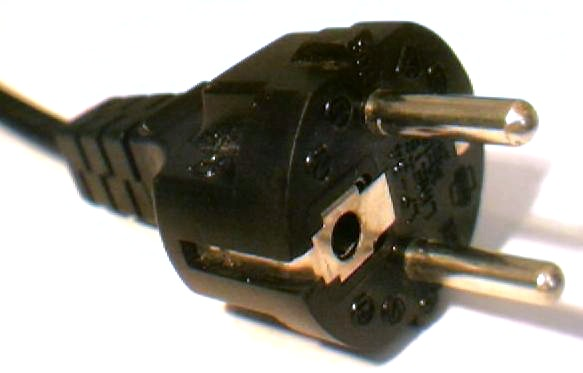
\includegraphics[width=0.6\textwidth]{images/plug}
    }
  \end{textblock}

\end{frame}

\begin{frame}[fragile]
  \frametitle{per-user rollback}

  \begin{semiverbatim}
\$ emacs --version
GNU Emacs \alert<5->{24.2}

\uncover<2->{\$ \alert<2>{guix package --upgrade emacs}
The following packages will be installed:
   emacs-\alert<2>{24.3.1}	out	/nix/store/...-emacs-24.3.1
...}

\uncover<3->{\$ \alert<3>{emacs --version}
Segmentation Fault}

\uncover<4->{\$ \alert<4>{guix package --roll-back}
switching from generation 43 to 42}

\uncover<5->{\$ \alert<5>{emacs --version}
GNU Emacs \alert<5->{24.2}
}
  \end{semiverbatim}

  \begin{textblock}{9}(10, 0)
    \only<1-2,4->{
\includegraphics[width=0.35\textwidth]{images/weather-clear}}
    \only<3>{
\includegraphics[width=0.35\textwidth]{images/weather-overcast}}
  \end{textblock}
\end{frame}

\subsection{foundations}

\begin{frame}
  \center{\huge{\textbf{functional package management}}}
  \\[2em]
  \begin{quote}
    \large{
    regarding the build \& installation process\\
    of a package as a \textbf{pure function}}
  \end{quote}
\end{frame}

% \begin{frame}
%   \frametitle{build environments \& reproducibility}

%   \vspace{-2cm}
%   \begin{itemize}
%     \item \alert{versions} of the dependencies
%     \item \alert{compiler}
%     \item \alert{compilation options}, and those of dependencies
%     \item \alert{miscellaneous} (locale, timezone, etc.)
%     \item \alert{paths}
%   \end{itemize}
%   \vspace{1.5cm}

%   \begin{textblock}{8}(2,8)
%     \uncover<2->{\texttt{-I/path/to/headers}}
%   \end{textblock}
%   \begin{textblock}{8}(10,8)
%     \uncover<2->{\texttt{\$CPATH}}
%   \end{textblock}

%   \begin{textblock}{8}(1,9)
%     \uncover<2->{\texttt{-L/path/to/lib}}
%   \end{textblock}
%   \begin{textblock}{8}(11,9)
%     \uncover<2->{\texttt{\$LIBRARY\_PATH}}
%   \end{textblock}

%   \begin{textblock}{8}(2,10)
%     \uncover<3->{\texttt{\$LD\_LIBRARY\_PATH}}
%   \end{textblock}
%   \begin{textblock}{8}(7,11)
%     \uncover<3->{\texttt{RPATH}}
%   \end{textblock}
%   \begin{textblock}{8}(12,11)
%     \uncover<3->{\texttt{RUNPATH}}
%   \end{textblock}

%   \begin{textblock}{8}(3,12)
%     \uncover<4->{\texttt{\$PYTHONPATH}}
%   \end{textblock}
%   \begin{textblock}{8}(7,13)
%     \uncover<4->{\texttt{\$PERL5LIB}}
%   \end{textblock}
%   \begin{textblock}{8}(1,13)
%     \uncover<4->{\texttt{\$XML\_CATALOG\_FILES}}
%   \end{textblock}
%   \begin{textblock}{8}(11,13)
%     \uncover<4->{\texttt{\$GUILE\_LOAD\_PATH}}
%   \end{textblock}
%   \begin{textblock}{8}(9,12)
%     \uncover<4->{\texttt{\$CLASSPATH}}
%   \end{textblock}

%   \begin{textblock}{8}(4,9)
%     \only<5->{
%       \tikz \node[fill=guixred1, inner sep=5mm, rotate=12,
%                   rounded corners=4]{
%         \textbf{ahem, reproducible builds?}
%       };
%     }
%   \end{textblock}

% \end{frame}

\begin{frame}
  \frametitle{controlling the build environment}
  \framesubtitle{... as pioneered by Nix}

  \begin{enumerate}
    \item<1-> one directory per installed package
    \item<2-> immutable installation directories
    \item<3-> undeclared dependencies invisible to the build process
    \item<4-> build performed in chroot, with separate UID, etc.
  \end{enumerate}

\end{frame}

\begin{frame}[fragile]
  \frametitle{the store}

  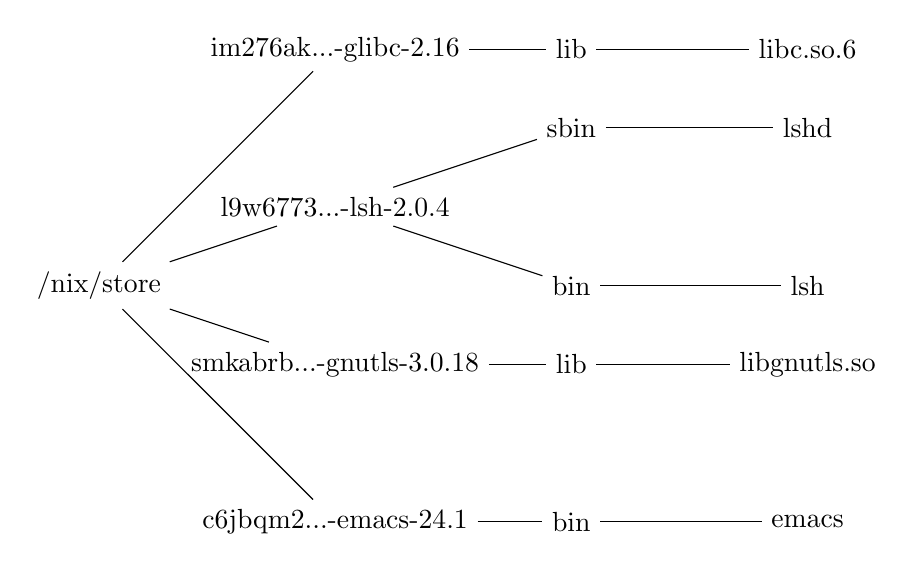
\begin{tikzpicture}
  
    \node {\alert{/nix/store}}
      %[edge from parent fork down, grow=right]
      [grow via three points={%
one child at (3,0) and two children at (3,-1) and (3,1)}]

      child {node {c6jbqm2...-\alert{emacs}-24.1}
        child {node {bin}
          child {node {emacs}}}}
      child {node {smkabrb...-\alert{gnutls}-3.0.18}
        child {node {lib}
          child {node {libgnutls.so}}}}
      child {node {l9w6773...-\alert{lsh}-2.0.4}
        child {node {bin}
          child {node {lsh}}}
        child {node {sbin}
          child {node {lshd}}}}
      child {node {im276ak...-\alert{glibc}-2.16}
        child {node {lib}
          child {node {libc.so.6}}}};

  \end{tikzpicture}
\end{frame}

\begin{frame}
  \frametitle{user environments}

  \begin{overlayarea}{\textwidth}{8cm}
    {
      \small
      \input{nix-user-envs.ltx}
    }

    \only<2-5>{\alert<2>{\code{guix package --upgrade openssh}}}
    % \only<6>{\alert{\code{nix-env --remove-generations old}}}
    \only<7>{\alert{\code{guix gc}}}

  \end{overlayarea}

\end{frame}

\begin{frame}[fragile]
  \frametitle{store file names}

  \begin{semiverbatim}
\$ guix build guile
\uncover<2->{/nix/store/\tikz[baseline]{\node[anchor=base](nixhash){\alert<2>{h2g4sc09h4...}};}-guile-2.0.9}

\uncover<3->{\$ \alert<3>{guix gc --references /nix/store/...-guile-2.0.9}
/nix/store/4jl83jgzaac...-glibc-2.17
/nix/store/iplay43cg58...-libunistring-0.9.3
/nix/store/47p47v92cj9...-libffi-3.0.9
/nix/store/drkwck2j965...-gmp-5.0.5
...}
  \end{semiverbatim}

  \begin{textblock}{7}(4, 10)
    \only<2>{\tikz{\node(labelnixhash)[fill=white, text=black]{hash of
          \emph{all} the dependencies};}}
  \end{textblock}

  % Arrows
  \only<2>{
    \begin{tikzpicture}[overlay]
      \path[->](labelnixhash.north) edge (nixhash.south);
    \end{tikzpicture}
  }

\end{frame}

\begin{frame}[fragile]
  \frametitle{complete dependency specification}

  \begin{overlayarea}{\textwidth}{6.5cm}
    \begin{center}
      \tikz \node(hellobuilddeps){\only<1-2>{\includegraphics[width=1.1\textwidth]{images/hello-buildtime-deps}}\only<3->{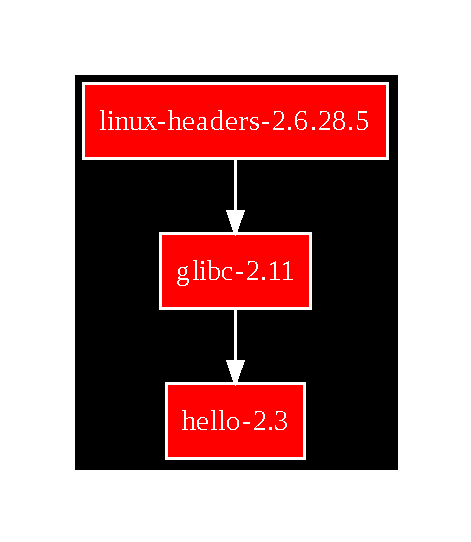
\includegraphics[width=0.5\textwidth]{images/hello-runtime-deps}}};
      \\
      \only<2>{\textbf{... down to the compiler's
          compiler!}}\uncover<3->{run-time dependencies inferred by
        \alert{conservative scanning}}
    \end{center}

    \begin{textblock}{6}(7, 2)
      \tikz \node(hellobuilddepslabel){\only<1-2>{build}\only<3->{run}-time dependencies of GNU Hello};
    \end{textblock}

    \begin{tikzpicture}[overlay]
      \only<1-2>{\path[->](hellobuilddepslabel.south) edge [bend left] (hellobuilddeps.north);}
    \end{tikzpicture}
  \end{overlayarea}
\end{frame}

\begin{frame}
  \frametitle{functional packaging summarized}

  \vspace{1cm}
  \begin{itemize}
    \item \alert{\bf immutable} software installations
    \item builds/installs have \alert{\bf no side effects}
    \item build \& deployment $\equiv$ calling the build function
    \item the store $\equiv$ \alert{\bf memoization}
    \item garbage collection...
  \end{itemize}
\end{frame}


\subsection{Nix's approach}

\begin{frame}[fragile]
  \frametitle{Nix is twofold}

  \begin{textblock}{7}(1, 3)
    \tikz \node[fill=white, text=black]{functional package deployment};
  \end{textblock}

  \begin{textblock}{7}(1, 5)
    \begin{itemize}
      \item the store
      \item file name hashes
      \item user environments
      \item transactional upgrades, etc.
      \item ...
    \end{itemize}
  \end{textblock}
  
  \only<2->{
    \begin{textblock}{7}(9, 3)
      \tikz \node[fill=white, text=black]{Nix packaging language};
    \end{textblock}

    \begin{textblock}{7}(8, 5)
      \begin{itemize}
      \item to describe package composition
      \item external DSL
      \item dynamically-typed, lazy
      \item easy integration of Bash snippets
      \item ...
      \end{itemize}
    \end{textblock}
  }
\end{frame}

\begin{frame}[fragile]
  \frametitle{Nix multi-user setup}

  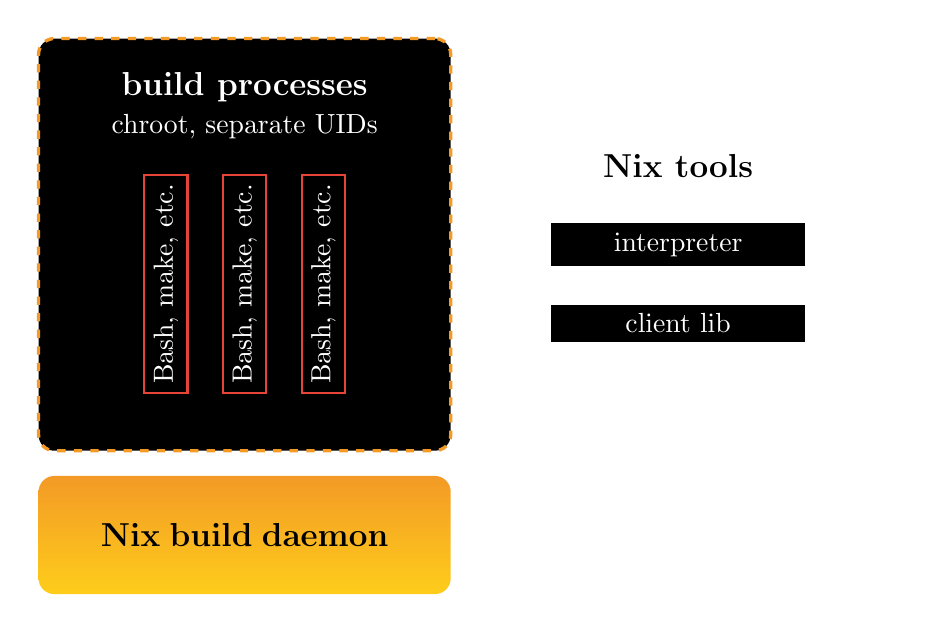
\begin{tikzpicture}[tools/.style = {
                        text width=35mm, minimum height=4cm,
                        text centered,
                        rounded corners=2mm,
                        fill=white, text=black
                      },
                      tool/.style = {
                        fill=black, text=white, text width=3cm,
                        text centered
                      },
                      daemon/.style = {
                        rectangle, text width=50mm, text centered,
                        rounded corners=2mm, minimum height=15mm,
                        top color=guixorange1,
                        bottom color=guixyellow,
                        text=black
                      },
                      builders/.style = {
                        draw=guixorange1, very thick, dashed,
                        fill=black, text=white, text width=5cm,
                        rounded corners=2mm,
                      },
                      builder/.style = {
                        draw=guixred2, thick, rectangle,
                        fill=black, text=white,
                        rotate=90
                      }]
    \matrix[row sep=3mm, column sep=1cm] {
      \node(builders)[builders, text height=5cm]{}
          node[fill=black, text=white] at (0, 2) {\large{\textbf{build processes}}}
          node[fill=black, text=white] at (0, 1.5) {chroot, separate UIDs}
          node[builder, onslide=<1-2>{black}] at (-1,-0.5) {Bash, make, etc.}
          node[builder, onslide=<1-2>{black}] at ( 0,-0.5) {Bash, make, etc.}
          node[builder, onslide=<1-2>{black}] at ( 1,-0.5) {Bash, make, etc.}; &
      \node[tools]{}
          node[fill=white, text=black] at (0, 1) {\large{\textbf{Nix tools}}}
          node[tool] at (0, 0) {interpreter}
          node(client)[tool] at (0, -1) {client lib};
      \\

      \node(daemon)[daemon]{\large{\textbf{Nix build daemon}}}; &
      &
      \\
    };
  \end{tikzpicture}

  \begin{tikzpicture}[overlay]
    \path[very thick, draw=guixorange1]<2->
      (client.south) edge [out=-90, in=0, ->] node[below, sloped]{RPCs} (daemon.east);
    \path[->, very thick, draw=guixorange1]<3->
      (daemon) edge (builders);
  \end{tikzpicture}
\end{frame}

\begin{frame}[fragile]
  \frametitle{Nix language build primitive}

  \small{
    \begin{semiverbatim}
\only<3->{\alert{let} dep = }\tikz[baseline]{\node[anchor=base](funcall){\alert{derivation}};} \{
  name = "foo";
  system = "x86\_64-linux";
  builder = "$\{./static-bash\}";
  args = [ "-c" "echo hello > "\tikz[baseline]{\node[anchor=base](outvar){$out};}" ];
\tikz[baseline]{\node[anchor=base](args){\}};}\uncover<3->{;}\uncover<3->{ in \alert{derivation} \{
  name = "bar";
  system = "x86\_64-linux";
  builder = "\$\{./static-bash\}";
  args = [ "-c"
    '' mkdir -p "$out"
       ln -s "\tikz[baseline]{\node[anchor=base](strinterp){\alert{$\{dep\}}};}/some-result" "\$out/my-result"
    '' ];
  PATH = "\$\{coreutils\}/bin";
\} }
    \end{semiverbatim}
  }

  \only<2>{
    \begin{textblock}{7}(6, 2)
      \tikz \node[fill=white, text=black](labelfuncall){function call};
    \end{textblock}

    \begin{textblock}{7}(11, 4)
      \tikz \node[fill=white, text=black](labeloutvar){\texttt{/nix/store/...-foo}};
    \end{textblock}

    \begin{textblock}{7}(5, 9)
      \tikz \node[fill=white, text=black](labelargs){named arguments};
    \end{textblock}

    \begin{tikzpicture}[overlay]
      \path[->](labelfuncall) edge (funcall);
      \path[->](labelargs) edge (args);
      \path[->](labeloutvar) edge [bend left] (outvar);
    \end{tikzpicture}
  }

  \only<4>{
    \begin{textblock}{7}(5,14)
      \tikz \node[fill=white, text=black](labelstrinterp){expands to \texttt{/nix/store/...-foo}};
    \end{textblock}

    \begin{tikzpicture}[overlay]
      \path[->](labelstrinterp) edge (strinterp);
    \end{tikzpicture}
  }
\end{frame}

\begin{frame}[fragile]
  \frametitle{Nix language high-level packaging}

  \vspace{1cm}
  \small{
    \begin{semiverbatim}
\{ \tikz[baseline]{\node[anchor=base](formalparams){fetchurl, stdenv};}\only<2->{, \alert{gettext}} \}\tikz[baseline]{\node[anchor=base](colon){:};}

\tikz[baseline]{\node[anchor=base](stdenv){\alert<2>{stdenv}};}.\tikz[baseline]{\node[anchor=base](funcall){\alert<1>{mkDerivation}};} \{
  name = "hello-2.3";
  src = fetchurl \{
    url = mirror://gnu/hello/hello-2.3.tar.bz2;
    sha256 = "0c7vijq8y68...";
  \};
 \uncover<2->{\tikz[baseline]{\node[anchor=base](dep){buildInputs = [ \alert{gettext} ];};}}
 \uncover<3->{\tikz[baseline]{\node[anchor=base](bash){preCheck = "echo 'Test suite coming up!'";};}}
  meta = \{
    description = "Produces a friendly greeting";
    homepage = http://www.gnu.org/software/hello/;
    license = "GPLv3+";
  \};
\}
    \end{semiverbatim}
    }

  \begin{textblock}{5}(10, 3)
    \tikz{\node<1>(labelcolon)[fill=white, text=black]{function definition};}
  \end{textblock}

  \begin{textblock}{5}(8, 5)
    \tikz{\node<1>(labelformalparams)[fill=white, text=black]{formal parameters};}
  \end{textblock}

  \begin{textblock}{5}(11, 6)
    \tikz{\node<1>(labelfuncall)[fill=white, text=black]{function call};}
  \end{textblock}

  \begin{textblock}{5}(10, 10)
    \tikz{\node<2>(labeldep)[fill=white, text=black]{dependency};}
  \end{textblock}

  \begin{textblock}{5}(5, 3)
    \tikz{\node<2>(labelstdenv)[fill=white, text=black]{\texttt{gcc}, \texttt{make}, etc.};}
  \end{textblock}

  \begin{textblock}{5}(11, 9)
    \tikz{\node<3>(labelbash)[fill=white, text=black]{Bash snippet};}
  \end{textblock}

  \begin{tikzpicture}[overlay]
    \path[->]<1>(labelcolon) edge (colon);
    \path[->]<1>(labelfuncall) edge (funcall);
    \path[->]<1>(labelformalparams) edge (formalparams);

    \path[->]<2>(labeldep) edge (dep);
    \path[->]<2>(labelstdenv) edge (stdenv);

    \path[->]<3>(labelbash) edge (bash);
  \end{tikzpicture}
\end{frame}

% \begin{frame}[fragile]
%   \frametitle{package composition with the Nix language}
%   \framesubtitle{\texttt{all-packages.nix}}

%   \vspace{1cm}
%   \begin{semiverbatim}
% \alert{gettext} = import ../development/libraries/gettext\tikz{\node(funcall2){};} \{
%   inherit \tikz[baseline]{\node[anchor=base](actualparams1){fetchurl stdenv libiconv;};}
% \};

% \textrm{...}

% \alert{hello} = import ../applications/misc/hello\tikz{\node(funcall3){};} \{
%   inherit \tikz[baseline]{\node[anchor=base](actualparams2){fetchurl stdenv};};
% \};
%   \end{semiverbatim}

%   \begin{textblock}{5}(5, 9)
%     \tikz{\node<1>(labelactualparams)[fill=white, text=black]{actual parameters};}
%   \end{textblock}

%   \begin{textblock}{5}(13, 9)
%     \tikz{\node<1>(labelfuncall2)[fill=white, text=black]{function call};}
%   \end{textblock}

%   \begin{tikzpicture}[overlay]
%     \path[->]<1->(labelactualparams) edge (actualparams1);
%     \path[->]<1->(labelactualparams) edge (actualparams2);
%     \path[->]<1->(labelfuncall2) edge (funcall2);
%     \path[->]<1->(labelfuncall2) edge (funcall3);
%   \end{tikzpicture}
% \end{frame}

\begin{frame}
  
  \vspace{3em}
  \huge{and now for parentheses...}

\end{frame}

%%%%%%%%%%%%%%%%%%%%%%%%%%%%%%%%%%%%%%%%%%%%%%%%%%%%%%%%%%%%%%%%%%%%%%%%%%%%%%%%
\section{from Nix to Guix}

\subsection{rationale}

\begin{frame}
  \frametitle{}

  \begin{quote}
    \Large{
      The truth is that Lisp is not the right language for any particular
      problem.  Rather, Lisp encourages one to attack a new problem by
      implementing new languages tailored to that problem.
    }
  \end{quote}

  \vspace{1cm}
  \hfill{-- Albelson \& Sussman, 1987}
\end{frame}

\begin{frame}
  \frametitle{from Nix\only<1>{...}\only<2->{ to Guix}}

  \begin{textblock}{7}(1, 3)
    \tikz \node[fill=white, text=black]{functional package deployment};
  \end{textblock}

  \begin{textblock}{7}(1, 5)
    \begin{itemize}
      \item the store
      \item file name hashes
      \item user environments
      \item transactional upgrades, etc.
      \item ...
    \end{itemize}
  \end{textblock}
  
  \begin{textblock}{7}(9, 3)
    \tikz \node[fill=white, text=black]{Nix packaging language};
  \end{textblock}

  \begin{textblock}{7}(8, 5)
    \begin{itemize}
    \item to describe package composition
    \item external DSL
    \item dynamically-typed, lazy
    \item easy integration of Bash snippets
    \item ...
    \end{itemize}
  \end{textblock}

  \begin{textblock}{5}(3,12)
    \only<2->{
      \tikz
      % \node[rotate=-5, drop shadow={shadow xshift=.8ex,shadow
      %   yshift=-.8ex}, fill=white, draw]{keep this}
      \node[overlay, rounded corners=4, text centered,
            minimum size=8mm, fill=guixorange1, text width=5cm,
            inner sep=3mm, rotate=0, opacity=.75, text opacity=1,
            drop shadow={opacity=0.5}] at (1, 0) {
              \textbf{reuse this}
            };
    }
  \end{textblock}

  \begin{textblock}{5}(11,3)
    \only<2->{
      \tikz
      \node[overlay, rounded corners=4, text centered,
            minimum size=8mm, fill=guixorange1, text width=5cm,
            inner sep=3mm, rotate=5, opacity=.75, text opacity=1,
            drop shadow={opacity=0.5}] at (1, 0) {
              \textbf{Scheme!}
            };

    }
  \end{textblock}
  
  \begin{textblock}{5}(11,10)
    \only<2->{
      \tikz
      \node[overlay, rounded corners=4, text centered,
            minimum size=10mm, fill=guixorange1, text width=5cm,
            inner sep=3mm, rotate=-4, opacity=.75, text opacity=1,
            drop shadow={opacity=0.5}] at (1, 0) {
              \textbf{Scheme!}
            };

    }
  \end{textblock}
\end{frame}

\begin{frame}[fragile]{Guix architecture}
  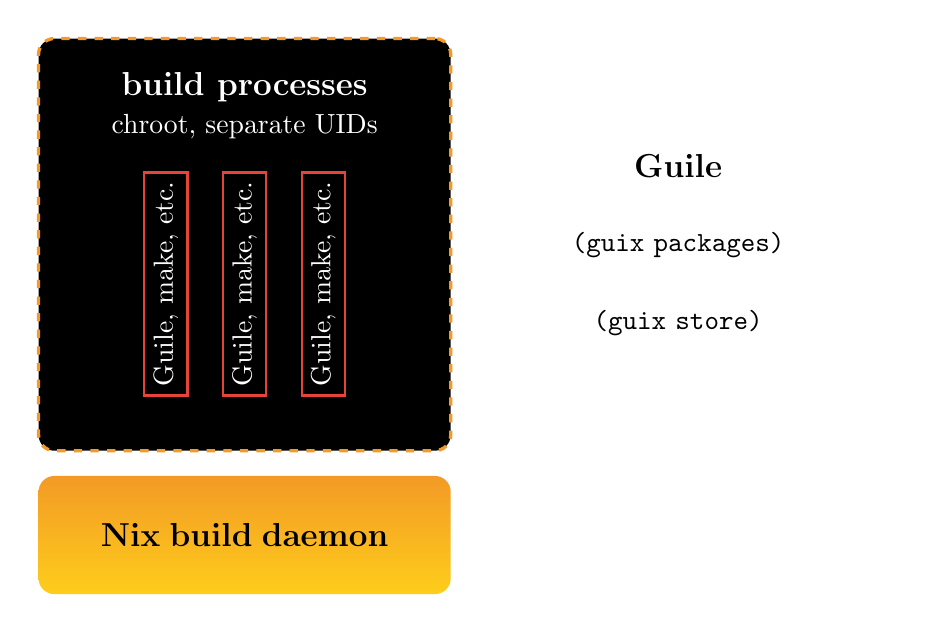
\begin{tikzpicture}[tools/.style = {
                        text width=35mm, minimum height=4cm,
                        text centered,
                        rounded corners=2mm,
                        fill=white, text=black
                      },
                      tool/.style = {
                        fill=white, text=black, text width=3cm,
                        text centered
                      },
                      daemon/.style = {
                        rectangle, text width=50mm, text centered,
                        rounded corners=2mm, minimum height=15mm,
                        top color=guixorange1,
                        bottom color=guixyellow,
                        text=black
                      },
                      builders/.style = {
                        draw=guixorange1, very thick, dashed,
                        fill=black, text=white, text width=5cm,
                        rounded corners=2mm,
                      },
                      builder/.style = {
                        draw=guixred2, thick, rectangle,
                        fill=black, text=white,
                        rotate=90
                      }]
    \matrix[row sep=3mm, column sep=1cm] {
      \node(builders)[builders, text height=5cm]{}
          node[fill=black, text=white] at (0, 2) {\large{\textbf{build processes}}}
          node[fill=black, text=white] at (0, 1.5) {chroot, separate UIDs}
          node[builder] at (-1,-0.5) {\alert{Guile}, make, etc.}
          node[builder] at ( 0,-0.5) {\alert{Guile}, make, etc.}
          node[builder] at ( 1,-0.5) {\alert{Guile}, make, etc.}; &
      \node[tools]{}
          node[fill=white, text=black] at (0, 1) {\large{\textbf{Guile}}}
          node[tool] at (0, 0) {\texttt{(guix packages)}}
          node(client)[tool] at (0, -1) {\texttt{(guix store)}};
      \\

      \node(daemon)[daemon]{\large{\textbf{Nix build daemon}}}; &
      &
      \\
    };
  \end{tikzpicture}

  \begin{tikzpicture}[overlay]
    \path[very thick, draw=guixorange1]
      (client.south) edge [out=-90, in=0, ->] node[below, sloped]{RPCs} (daemon.east);
    \path[->, very thick, draw=guixorange1]
      (daemon) edge (builders);
  \end{tikzpicture}
\end{frame}

\begin{frame}{thesis}

  \Large{
    \begin{enumerate}
    \item Scheme + EDSL at least as \alert{expressive} as the Nix
      language
    \item Scheme better suited than the shell for \alert{build
        programs}
    \item Guix provides a \alert{unified \& extensible} programming
      environment
    \end{enumerate}
  }    
\end{frame}

\subsection{programming interfaces}

\begin{frame}{programming interface layers}

  \large{
    \begin{enumerate}
    \item \alert{\textbf{declarative}} packaging layer
    \item Scheme \alert{\textbf{build expressions}}
    \item \alert{\texttt{derivation}} primitive (from Nix)
    \end{enumerate}
  }
\end{frame}

\begin{frame}[fragile]{declarative packaging layer}
  \begin{semiverbatim}
    \small{
(define hello
  (\alert{package}
   (name "hello")
   (version "2.8")
   (source (\alert{origin}
            (method url-fetch)
            (uri (string-append
                  "http://ftp.gnu.org/\textrm{...}/hello-" version
                  ".tar.gz"))
            (sha256 (base32 "0wqd\textrm{...}dz6"))))
   (\alert{build-system} gnu-build-system)
   (synopsis "GNU Hello")
   (description "Produce a friendly greeting.")
   (home-page "http://www.gnu.org/software/hello/")
   (license gpl3+)))
}
  \end{semiverbatim}

  \begin{textblock}{15}(6,7)
    \only<2>{
      \tikz
      \node[overlay, rounded corners=4, text centered,
      minimum size=10mm, fill=guixorange1, text width=5cm,
      inner sep=2mm, rotate=-3, opacity=.75, text opacity=1,
      drop shadow={opacity=0.5}] at (1, 0) {
        \textbf{how do we reach this level of abstraction?}
      };
    }
  \end{textblock}
\end{frame}

\begin{frame}[fragile]{Nix's \texttt{derivation} primitive in Scheme}
  \begin{semiverbatim}
(let* ((store \tikz[baseline]{\node[anchor=base](conn){(open-connection)};})
       (bash  (\tikz[baseline]{\node[anchor=base](addtostore){add-to-store};} store "static-bash"
                            #t "sha256"
                            "./static-bash")))
  (\tikz[baseline]{\node[anchor=base](derivation){\alert{derivation}};} store "example-1.0" 
              "x86\_64-linux" 
              \tikz[baseline]{\node[anchor=base](bash){bash};}
              '("-c" "echo hello > \$out")
              '(("HOME" . "/homeless"))
              '()))

=> "/nix/store/nsswy...-example-1.0\tikz[baseline]{\node[anchor=base](drv){.drv};}"
=> \#<derivation "example-1.0" ...>
  \end{semiverbatim}

  \only<2>{
    \begin{textblock}{6}(7, 2)
      \tikz{\node<2>[fill=white, text=black](labelconn){connect to
          the build daemon};}
    \end{textblock}

    \begin{tikzpicture}[overlay]
      \path[->, fill=white, thick]<2>(labelconn) edge (conn);
    \end{tikzpicture}
  }

  \only<3>{
    \begin{textblock}{5}(11, 3)
      \tikz \node[fill=white, text=black](labeladdtostore){``intern''
        the file};
    \end{textblock}
    
    \begin{textblock}{6}(8, 8)
      \tikz \node[fill=white,
      text=black](labelbash){\texttt{/nix/store/...-static-bash}};
    \end{textblock}

    \begin{tikzpicture}[overlay]
      \path[->, thick] (labeladdtostore) edge (addtostore);
      \path[->, thick] (labelbash) edge (bash);
    \end{tikzpicture}
  }

  \only<4>{
    \begin{textblock}{5}(1, 9)
      \tikz{\node[fill=white, text=black, text
        width=4.0cm](labeldrv){compute ``derivation''---i.e., build
          promise};}
    \end{textblock}

    \begin{tikzpicture}[overlay]
      \path[->, thick] (labeldrv) edge (derivation);
      \path[->, thick] (labeldrv) edge (drv);
    \end{tikzpicture}
  }
\end{frame}

\begin{frame}[fragile]{build expressions}
  \begin{semiverbatim}
(let* ((store   \tikz[baseline]{\node[anchor=base](conn){(open-connection)};})
       (builder '(\tikz[baseline]{\node[anchor=base](builder){begin};}
                   (mkdir \%output)
                   (call-with-output-file
                       (string-append \%output "/test")
                     (lambda (p)
                       (display '(hello guix) p)))))
       (drv (\tikz[baseline]{\node[anchor=base](drv){\alert{build-expression->derivation}};}
               store "foo" "x86\_64-linux"
               builder
               '(("HOME" . "/nowhere")))))
  (\tikz[baseline]{\node[anchor=base](build){\alert{build-derivations}};} store (list drv)))
  \end{semiverbatim}

  % \begin{textblock}{6}(3, 2)
  %   \tikz{\node<2>[fill=white, text=black](labelconn){connect to
  %       the build daemon};}
  % \end{textblock}

  \begin{textblock}{6}(8, 2)
    \tikz{\node<2>[fill=white, text=black](labelbuilder){build script,
        to be eval'd in chroot};}
  \end{textblock}

  \begin{textblock}{4}(1, 6)
    \tikz{\node<3>[fill=white, text=black, text width=4cm](labeldrv){compute derivation
        for this builder, system, and env.~vars};}
  \end{textblock}

  \begin{textblock}{5}(1, 7)
    \tikz{\node<4>[fill=white, text=black, text
      width=4cm](labelguile){implicitly adds Guile as an input};}
  \end{textblock}

  \begin{textblock}{6}(1, 9)
    \tikz{\node<5>[fill=white, text=black](labelbuild){build it!};}
  \end{textblock}

  \begin{tikzpicture}[overlay]
    % \path[->, fill=white, thick]<2>(labelconn) edge (conn);
    \path[->, fill=white, thick]<2>(labelbuilder) edge (builder);
    \path[->, fill=white, thick]<3>(labeldrv) edge (drv);
    \path[->, fill=white, thick]<4>(labelguile) edge (drv);
    \path[->, fill=white, thick]<5>(labelbuild) edge (build);
  \end{tikzpicture}
\end{frame}

\begin{frame}[fragile]{declarative packaging layer}
  \begin{semiverbatim}
    \vspace{-0.8cm}
    \small{
(define hello
  (\alert{package}
   (name "hello")
   (version "2.8")
   (source (\alert{origin}
            (method url-fetch)
            (uri (string-append
                  "http://ftp.gnu.org/\textrm{...}/hello-" version
                  ".tar.gz"))
            (sha256 (base32 "0wqd\textrm{...}dz6"))))
   (\alert{build-system} \tikz[baseline]{\node[anchor=base](gbs){gnu-build-system};})
   \tikz[baseline]{\node[anchor=base](deps){(inputs `(("gawk" ,\tikz[baseline]{\node[anchor=base](gawkvar){\only<1-3,5->{\alert<3>{gawk}}\only<4>{\alert{my-other-awk}}};})))};}
   (synopsis "GNU Hello")
   (description "Produce a friendly greeting.")
   (home-page "http://www.gnu.org/software/hello/")
   (license gpl3+)))
}
  \end{semiverbatim}

  \begin{textblock}{5}(11, 12)
    \tikz{\node<2-3>(labeldeps)[fill=white, text=black]{dependencies};}
  \end{textblock}

  \begin{textblock}{5}(9, 9)
    \tikz{\node<3-4>(labelgawkvar)[fill=white, text=black]{reference to a
        variable};}
  \end{textblock}

  \begin{textblock}{5}(3, 5)
    \tikz{\node<5>(labelgbs)[fill=white, text=black]{\texttt{./configure
        \&\& make install}...};}
  \end{textblock}

  \begin{textblock}{5}(8, 7)
    \tikz{\node<5>(labelgbsdeps)[fill=white, text=black]{depends on
        \texttt{gcc}, \texttt{make}, \texttt{bash}, etc.};}
  \end{textblock}

  \begin{tikzpicture}[overlay]
    \path[->, fill=white, thick]<2-3>(labeldeps) edge (deps);
    \path[->, fill=white, thick]<3-4>(labelgawkvar) edge (gawkvar);
    \path[->, fill=white, thick]<5>(labelgbs) edge (gbs);
    \path[->, fill=white, thick]<5>(labelgbsdeps) edge (gbs);
  \end{tikzpicture}
\end{frame}

\begin{frame}[fragile]{build-system protocol}
  \begin{semiverbatim}
(define gnu-build-system
  (\alert{build-system} (name 'gnu)
    (description "./configure \&\& make \&\& make install")
    (build gnu-build)
    (cross-build gnu-cross-build)))
  \end{semiverbatim}

  \begin{itemize}
    \item<2-> \texttt{python-build-system}: run \texttt{python setup.py}
      etc.
    \item<2-> \texttt{perl-build-system}: run \texttt{perl Makefile.PL}
      etc.
    \item<2-> \texttt{cmake-build-system}: run \texttt{cmake .} etc.
  \end{itemize}
\end{frame}

\begin{frame}[fragile]{building packages}
  \begin{semiverbatim}
(\alert{use-modules} (guix packages) (guix store)
             (gnu packages base))

(define store
  \tikz[baseline]{\node[anchor=base](conn){(\alert<1>{open-connection})};})

(package? hello)
=> \#t

\uncover<2->{(define drv (\tikz[baseline]{\node[anchor=base](drv){\alert<2>{package-derivation}};} store hello))
\uncover<3->{drv
=> "/nix/store/xyz\textrm{...}-hello-2.8\alert<3>{.drv}"

\uncover<4->{(build-derivations (list drv))
\textsf{\alert{... daemon builds/downloads package on our behalf...}}
\uncover<5->{=> "/nix/store/pqr\textrm{...}-hello-2.8"}}}}
  \end{semiverbatim}

  \begin{textblock}{6}(8, 4)
    \tikz{\node<1>[fill=white, text=black](labelconn){connect to
        the Nix build daemon};}
  \end{textblock}

  \begin{textblock}{6}(9, 6)
    \tikz{\node<2>[fill=white, text=black, text
      width=4.3cm](labeldrv){compute ``derivation''---i.e., build
        promise};}
  \end{textblock}

  \begin{tikzpicture}[overlay]
    \path[->, fill=white, thick]<1>(labelconn) edge (conn);
    \path[->, fill=white, thick]<2>(labeldrv) edge (drv);
  \end{tikzpicture}
\end{frame}

\begin{frame}[fragile]{building packages}
  \begin{semiverbatim}
\$ \alert<1>{guix build}\only<3->{ --\alert{target}=armel-linux-gnueabi} hello
\uncover<2->{The following derivations will be built:
   /nix/store/\only<1-2>{4gy79}\only<3>{1gm99}\textrm{...}-\only<1-2>{gawk-4.0.0}\only<3>{gcc-armel-linux-gnu-4.8.1}.drv
   /nix/store/\only<1-2>{7m2r9}\only<3>{71ah1}\textrm{...}-hello-2.8.drv
\textrm{...}
\alert{/nix/store/\only<1-2>{71aj1}\only<3->{7m2r9}\textrm{...}-hello-2.8}
}
\end{semiverbatim}
\end{frame}

% \begin{frame}[fragile]{customized package declaration}
%   \begin{semiverbatim}
%     \vspace{-1.3cm}
%     \small{
% (define guile-1.8
%   (\alert{package} \textrm{...}
%    (\alert{arguments}
%      '(\alert<1>{#:configure-flags} '("--disable-error-on-warning")
%        \uncover<2->{\alert<2>{#:patches} (list (assoc-ref %build-inputs "patch/snarf"))}

%        \uncover<3->{
%        \alert<3-4>{#:phases}
%          (\tikz[baseline]{\node[anchor=base](alistcons){alist-cons-before 'configure 'patch-search-path};}
%             (lambda* (#:key outputs #:allow-other-keys)
%               (\tikz[baseline]{\node[anchor=base](subst){\alert<5>{substitute*}};} "libguile/dynl.c"
%                 (("lt_dlinit.*\$" match)
%                  (format \#f
%                    "  ~a~\%  lt\_dladdsearchdir(\\"~a/lib\\");~\%"
%                    match (assoc-ref outputs "out")))))
%             \tikz[baseline]{\node[anchor=base](phases){\alert<3-4>{\%standard-phases}};})}))
%    (inputs `(\uncover<2->{("\alert<2>{patch/snarf}" "guile-1.8.patch")}
%              ("gawk" ,gawk)
%              ("readline" ,readline)))

%    ...
%    }
%   \end{semiverbatim}

%   \begin{textblock}{5}(1, 9)
%     \tikz{\node<3-4>[fill=white, text=black](labelphases){configure, build, check, install};}
%   \end{textblock}

%   \begin{textblock}{5}(8, 5)
%     \tikz{\node<4>(labelalistcons)[fill=white, text=black]{add a phase
%         before \texttt{configure}};}
%   \end{textblock}

%   \begin{textblock}{5}(5, 5)
%     \tikz{\node<5>(labelsubst)[fill=white, text=black]{patch things up à
%         la \texttt{sed}};}
%   \end{textblock}

%   \begin{tikzpicture}[overlay]
%     \path[->, fill=white, thick]<3-4>(labelphases) edge (phases);
%     \path[->, fill=white, thick]<4>(labelalistcons) edge (alistcons);
%     \path[->, fill=white, thick]<5>(labelsubst) edge (subst);
%   \end{tikzpicture}
% \end{frame}

\begin{frame}[fragile]{packages based on existing ones}
  \begin{semiverbatim}
(package (\tikz[baseline]{\node(inherit)[anchor=base]{\alert{inherit}};} hello)
  (version "2.7")
  (source
    (origin
      (method url-fetch)
      (uri "mirror://gnu/hello/hello-2.7.tar.gz")
      (sha256
        (base32 "7dqw3...")))))
  \end{semiverbatim}

  \begin{textblock}{6}(7, 2)
    \tikz \node(labelinherit)[fill=white, text=black, text width=5.5cm]
      {copy fields from \texttt{hello} except for \texttt{version} and
        \texttt{source}};
  \end{textblock}
  
  \begin{tikzpicture}[overlay]
    \path[->] (labelinherit) edge (inherit);
  \end{tikzpicture}
\end{frame}

\begin{frame}[fragile]{functional package adapters}
  \begin{semiverbatim}
(define (static-package p)
  ;; Return a statically-linked variant of P.
  (package (\alert{inherit} p)
    (arguments
     `(\#:configure-flags '("--disable-shared"
                            "LDFLAGS=-static")
       ,@(package-arguments p)))))
  \end{semiverbatim}
\end{frame}

% \begin{frame}[fragile]{system-dependent inputs}
% \end{frame}

\begin{frame}[fragile]{system-dependent arguments}
  \begin{semiverbatim}
    \vspace{-1.3cm}
    \small{
(define gawk
  (\alert{package}
   (name "gawk")
   (version "4.0.2")
   (source (origin (method url-fetch)
                   (uri "http://ftp.gnu.org/...")
                   (sha256 (base32 "0sss..."))))
   (build-system gnu-build-system)
   (\alert{arguments}
     (if (string-prefix? "i686" (\tikz[baseline]{\node[anchor=base](sys){\%current-system};}))
         '(#:tests? #f)      ; skip tests on 32-bit hosts
         '()))
   (inputs `(("libsigsegv" ,libsigsegv)))
   (home-page "http://www.gnu.org/software/gawk/")
   (synopsis "GNU Awk")))
   }
 \end{semiverbatim}

  \begin{textblock}{5}(9, 5)
    \tikz \node<2>(labelsys)
           [fill=white, text=black, text width=4cm]
           {dynamically-scoped parameter (SRFI-39)};
  \end{textblock}


  \begin{tikzpicture}[overlay]
    \node<2> [fill=white, text=black, text opacity=1, opacity=.7,
              rounded corners=2mm, inner sep=3mm, text width=5.5cm]
             at (120pt, 44pt)
             {evaluated within the dynamic extent of \texttt{package-derivation}};
    \draw<2> (16pt, 110pt) [very thick, color=guixorange2, rounded corners=8pt]
      arc (20:-40:-40pt and 45pt);
    \path[->, fill=white, thick]<2>(labelsys) edge (sys);
  \end{tikzpicture}
\end{frame}

\begin{frame}[fragile]{under the hood: fancy records}
  \vspace{-0.3cm}
  \begin{semiverbatim}
(\alert{define-record-type*} <package>
  \tikz[baseline]{\node(package)[anchor=base]{package};} make-package package?

  (name package-name)
  (version package-version)
  (source package-source)
  (build-system package-build-system)
  (arguments package-arguments
             (\alert{default} '()) (\tikz[baseline]{\node(thunked)[anchor=base]{\alert{thunked}};}))

  (inputs package-inputs
          (\alert{default} '()) (\alert{thunked}))

  ;; \ldots{}

  (location package-location
     (\alert{default} (current-source-location))))
  \end{semiverbatim}

  \begin{textblock}{6}(9, 5)
    \tikz \node<2>(labelthunked)
      [fill=white, text=black]
      {enclose value in a thunk};
  \end{textblock}
  
  \begin{textblock}{6}(10, 3)
    \tikz \node<2>(labelpackage)[fill=white, text=black]{generated
      macro};
  \end{textblock}
  
  \begin{tikzpicture}[overlay]
    \path[->, fill=white, thick]<2> (labelthunked) edge (thunked);
    \path[->, fill=white, thick]<2> (labelpackage.west)
      edge [bend left, out=0, in=165] (package);
  \end{tikzpicture}
\end{frame}

\subsection{builder-side code}

\begin{frame}[fragile]{builder side of \texttt{gnu-build-system}}
  \vspace{-0.4cm}
  \begin{semiverbatim}
(\alert{define} \%standard-phases
  `((configure . ,configure)
    (build . ,build)
    ;; \textrm{...}
    ))

(\alert{define*} (gnu-build #:key (phases \%standard-phases)
                    #:allow-other-keys
                    #:rest args)
  ;; Run all the PHASES in order, passing them ARGS.
  (every (match-lambda
          ((name . proc)
           (format #t "starting phase `~a'~\%" name)
           (let ((result (apply proc args)))
             (format #t "phase `~a' done~\%" name)
             result)))
         phases))
  \end{semiverbatim}
\end{frame}

\begin{frame}[fragile]{inserting a build phase}
  \begin{semiverbatim}
(define howdy
  (\alert{package} (inherit hello)
    (arguments
      '(#:phases
        (\tikz[baseline]{\node(alistcons)[anchor=base]{alist-cons-after};}
          'configure 'change-hello
          (lambda* (#:key system #:allow-other-keys)
            (\tikz[baseline]{\node(subst)[anchor=base]{\alert<4>{substitute*}};} "src/hello.c"
              (("Hello, world!")
               (string-append "Howdy! Running on "
                              system "."))))
          \tikz[baseline]{\node(phases)[anchor=base]{\%standard-phases};})))))
  \end{semiverbatim}

  \begin{tikzpicture}[overlay]
    \draw<2> (40pt, 145pt) [very thick, color=guixorange2, rounded corners=8pt]
      arc (20:-40:-50pt and 110pt);
    \node<2>[fill=white, text=black, text opacity=1, opacity=.7,
          rounded corners=2mm, inner sep=5mm]
      at (7, 4) {\textbf{builder-side expression}};
  \end{tikzpicture}

  \begin{textblock}{5}(1, 9)
    \tikz{\node<3>[fill=white, text=black](labelphases){configure, build, check, install};}
  \end{textblock}

  \begin{textblock}{5}(8, 5)
    \tikz{\node<3>(labelalistcons)[fill=white, text=black]{add a phase
        before \texttt{configure}};}
  \end{textblock}

  \begin{textblock}{5}(5, 5)
    \tikz{\node<4>(labelsubst)[fill=white, text=black]{patch things up à
        la \texttt{sed}};}
  \end{textblock}

  \begin{tikzpicture}[overlay]
    \path[->, fill=white, thick]<3>(labelphases) edge (phases);
    \path[->, fill=white, thick]<3>(labelalistcons) edge (alistcons);
    \path[->, fill=white, thick]<4>(labelsubst) edge (subst);
  \end{tikzpicture}
\end{frame}

\begin{frame}[fragile]{downloading sources}
  \begin{semiverbatim}
(\alert{origin}
  (method \tikz[baseline]{\node(fetch)[anchor=base]{url-fetch};})
  (uri (string-append "mirror://gnu/gcc/gcc-"
                      version "/gcc-" version
                      ".tar.bz2"))
  (sha256 (base32 "1hx9\textrm{...}")))
  \end{semiverbatim}

  \begin{tikzpicture}[overlay]
    \node<2->(labelfetch)[fill=white, text=black] at (4, 5)
      {use Guile HTTP(S)/FTP client};
    \path[->, fill=white, thick]<2-> (labelfetch) edge (fetch);

    \node<3->[overlay, rounded corners=4, text centered,
            minimum size=10mm, fill=guixorange1, text width=5cm,
            inner sep=3mm, rotate=2, opacity=.75, text opacity=1,
            drop shadow={opacity=0.5}] at (5, 1) {
              \textbf{how is the very first tarball downloaded?}
            };
  \end{tikzpicture}
\end{frame}

\begin{frame}[fragile]{bootstrapping the distribution}
  \begin{enumerate}
    \setcounter{enumi}{0}
    \item statically-linked binaries of \texttt{mkdir}, \texttt{tar},
      \texttt{xz}, \texttt{bash}, and Guile
    \item run Bash script to untar Guile
    \item use Guile to download statically-linked binaries of GCC,
      Binutils, libc, Coreutils et al., and Bash
    \item use that to build GNU~Make
    \item ...
  \end{enumerate}
\end{frame}

\section{evaluation \& discussion}

\begin{frame}{status}
  \begin{itemize}
  \item API/language support for builds \& composition
  \item builder-side libs equiv. to \texttt{wget}, \texttt{find},
    \texttt{grep}, \texttt{sed}, etc.
  \item expressive enough to build a variety of packages
  \end{itemize}
\end{frame}

\begin{frame}{benefits of DSL embedding}
  \begin{enumerate}
    \item{Guile tools readily available
        \begin{itemize}
          \item<2-> libraries, macros, compiler, etc.
          \item<2-> i18n support (for package descriptions)
          \item<2-> development environment: Emacs + Geiser
        \end{itemize}}
    \item{simplified implementation of auxiliary tools
        \begin{itemize}
          \item<2-> off-line \& on-line package auto-updater
          \item<2-> description synchronization with external DB
          \item<2-> searching packages by keyword
        \end{itemize}}
  \end{enumerate}
\end{frame}

\begin{frame}{GNU/Linux distribution}
  \begin{itemize}
    \item installable atop a running GNU/Linux system
    \item self-contained (pure!)
    \item transactional upgrade/roll-back, pre-built binaries, etc.
    \item {$\approx$400 packages
        \begin{itemize}
          \item TeX Live, Xorg, GCC, ...
          \item and 6 Scheme implementations! :-)
        \end{itemize}}
  \end{itemize}
\end{frame}

\begin{frame}[fragile]{pushing the limits: booting to Guile}
  \vspace{-0.7cm}
  \begin{semiverbatim}
\small{
(\alert{expression->initrd}
 '(begin
    (mkdir "/proc")
    (mount "none" "/proc" "proc")

    ;; Load Linux kernel modules.
    (let ((slurp (lambda (module)
                   (call-with-input-file
                       (string-append "/modules/" module)
                     get-bytevector-all))))
      (for-each (compose load-linux-module slurp)
                (list "md4.ko" "ecb.ko" "cifs.ko")))

    ;; Turn eth0 up.
    (let ((sock (socket AF_INET SOCK_STREAM 0)))
      (set-network-interface-flags sock "eth0" IFF_UP))

    ;; At last, the warm and friendly REPL.
    (start-repl)))
}
  \end{semiverbatim}
\end{frame}

\begin{frame}{road map}
  \begin{itemize}
    \item{ \alert{short-term}
        \begin{itemize}
          \item tweak more packages for cross-compilation
          \item port to mips64el (N64), and armel (?)
          \item more packages: GTK+ stack, applications
          \end{itemize}}
    \item<2->{ \alert{medium-term}
        \begin{itemize}
          \item stand-alone, bootable distribution!
          \item with NixOS-style whole-system configuration EDSL
          \item with the Guile-powered DMD init system
        \end{itemize}}
  \end{itemize}

  \begin{textblock}{5}(7,8)
    \tikz
    \node<3->[overlay, rounded corners=4, text centered,
            minimum size=10mm, fill=guixorange1, text width=5cm,
            inner sep=3mm, rotate=4, opacity=.75, text opacity=1,
            drop shadow={opacity=0.5}] at (1, 0) {
              \textbf{Your help needed!}
            };

  \end{textblock}
\end{frame}

\begin{frame}{no compromise}
  \center{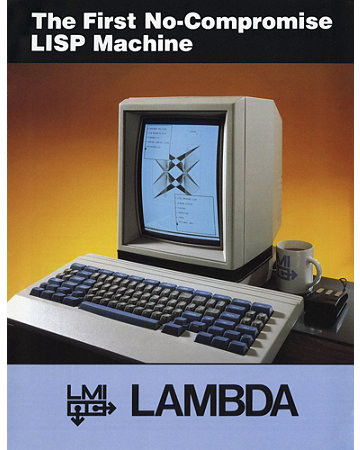
\includegraphics[width=0.6\textwidth]{images/lmi-machine}}
  \\
\end{frame}

\begin{frame}
  \frametitle{summary}

  \begin{itemize}
  \item \textbf{features}
    \begin{itemize}
    \item transactional upgrades; rollback; per-user profiles
    \item full power of Guile to build \& compose packages
    \item unified packaging development environment
    \end{itemize}
  \item \textbf{foundations}
    \begin{itemize}
    \item purely functional package management
    \item packaging DSL embedded in Scheme
    \item second tier: flexible builds programs in Scheme
    \end{itemize}
  \end{itemize}
\end{frame}

\begin{frame}{}

\vfill{
  \vspace{6.5cm}
  \hfill{
\includegraphics[width=0.3\textwidth]{images/guix-logo-white}}\\[0.2cm]
  \texttt{ludo@gnu.org} \hfill{\alert{\url{http://gnu.org/software/guix/}}}
}

\end{frame}

\begin{frame}{}

  \begin{textblock}{12}(2, 8)
    \tiny{
      Copyright \copyright{} 2010, 2012, 2013 Ludovic Courtès \texttt{ludo@gnu.org}.

      Picture of user environments is: \\
      Copyright \copyright{} 2009 Eelco Dolstra \texttt{e.dolstra@tudelft.nl}.

      Copyright of other images included in this document is held by
      their respective owners.
      \\[3.0mm]
      This work is licensed under the \alert{Creative Commons
        Attribution-Share Alike 3.0} License.  To view a copy of this
      license, visit
      \url{http://creativecommons.org/licenses/by-sa/3.0/} or send a
      letter to Creative Commons, 171 Second Street, Suite 300, San
      Francisco, California, 94105, USA.
      \\[2.0mm]
      At your option, you may instead copy, distribute and/or modify
      this document under the terms of the \alert{GNU Free Documentation
        License, Version 1.3 or any later version} published by the Free
      Software Foundation; with no Invariant Sections, no Front-Cover
      Texts, and no Back-Cover Texts.  A copy of the license is
      available at \url{http://www.gnu.org/licenses/gfdl.html}.
      \\[2.0mm]
      % Give a link to the 'Transparent Copy', as per Section 3 of the GFDL.
      The source of this document is available from
      \url{http://git.sv.gnu.org/cgit/guix/maintenance.git}.
    }
  \end{textblock}
\end{frame}


\end{document}

% Local Variables:
% coding: utf-8
% comment-start: "%"
% comment-end: ""
% ispell-local-dictionary: "american"
% compile-command: "rubber --pdf guix-els-2013.tex"
% End:
